\documentclass[twoside]{book}

% Packages required by doxygen
\usepackage{fixltx2e}
\usepackage{calc}
\usepackage{doxygen}
\usepackage[export]{adjustbox} % also loads graphicx
\usepackage{graphicx}
\usepackage[utf8]{inputenc}
\usepackage{makeidx}
\usepackage{multicol}
\usepackage{multirow}
\PassOptionsToPackage{warn}{textcomp}
\usepackage{textcomp}
\usepackage[nointegrals]{wasysym}
\usepackage[table]{xcolor}

% Font selection
\usepackage[T1]{fontenc}
\usepackage[scaled=.90]{helvet}
\usepackage{courier}
\usepackage{amssymb}
\usepackage{sectsty}
\renewcommand{\familydefault}{\sfdefault}
\allsectionsfont{%
  \fontseries{bc}\selectfont%
  \color{darkgray}%
}
\renewcommand{\DoxyLabelFont}{%
  \fontseries{bc}\selectfont%
  \color{darkgray}%
}
\newcommand{\+}{\discretionary{\mbox{\scriptsize$\hookleftarrow$}}{}{}}

% Page & text layout
\usepackage{geometry}
\geometry{%
  a4paper,%
  top=2.5cm,%
  bottom=2.5cm,%
  left=2.5cm,%
  right=2.5cm%
}
\tolerance=750
\hfuzz=15pt
\hbadness=750
\setlength{\emergencystretch}{15pt}
\setlength{\parindent}{0cm}
\setlength{\parskip}{3ex plus 2ex minus 2ex}
\makeatletter
\renewcommand{\paragraph}{%
  \@startsection{paragraph}{4}{0ex}{-1.0ex}{1.0ex}{%
    \normalfont\normalsize\bfseries\SS@parafont%
  }%
}
\renewcommand{\subparagraph}{%
  \@startsection{subparagraph}{5}{0ex}{-1.0ex}{1.0ex}{%
    \normalfont\normalsize\bfseries\SS@subparafont%
  }%
}
\makeatother

% Headers & footers
\usepackage{fancyhdr}
\pagestyle{fancyplain}
\fancyhead[LE]{\fancyplain{}{\bfseries\thepage}}
\fancyhead[CE]{\fancyplain{}{}}
\fancyhead[RE]{\fancyplain{}{\bfseries\leftmark}}
\fancyhead[LO]{\fancyplain{}{\bfseries\rightmark}}
\fancyhead[CO]{\fancyplain{}{}}
\fancyhead[RO]{\fancyplain{}{\bfseries\thepage}}
\fancyfoot[LE]{\fancyplain{}{}}
\fancyfoot[CE]{\fancyplain{}{}}
\fancyfoot[RE]{\fancyplain{}{\bfseries\scriptsize Generated by Doxygen }}
\fancyfoot[LO]{\fancyplain{}{\bfseries\scriptsize Generated by Doxygen }}
\fancyfoot[CO]{\fancyplain{}{}}
\fancyfoot[RO]{\fancyplain{}{}}
\renewcommand{\footrulewidth}{0.4pt}
\renewcommand{\chaptermark}[1]{%
  \markboth{#1}{}%
}
\renewcommand{\sectionmark}[1]{%
  \markright{\thesection\ #1}%
}

% Indices & bibliography
\usepackage{natbib}
\usepackage[titles]{tocloft}
\setcounter{tocdepth}{3}
\setcounter{secnumdepth}{5}
\makeindex

% Hyperlinks (required, but should be loaded last)
\usepackage{ifpdf}
\ifpdf
  \usepackage[pdftex,pagebackref=true]{hyperref}
\else
  \usepackage[ps2pdf,pagebackref=true]{hyperref}
\fi
\hypersetup{%
  colorlinks=true,%
  linkcolor=blue,%
  citecolor=blue,%
  unicode%
}

% Custom commands
\newcommand{\clearemptydoublepage}{%
  \newpage{\pagestyle{empty}\cleardoublepage}%
}

\usepackage{caption}
\captionsetup{labelsep=space,justification=centering,font={bf},singlelinecheck=off,skip=4pt,position=top}

%===== C O N T E N T S =====

\begin{document}

% Titlepage & ToC
\hypersetup{pageanchor=false,
             bookmarksnumbered=true,
             pdfencoding=unicode
            }
\pagenumbering{alph}
\begin{titlepage}
\vspace*{7cm}
\begin{center}%
{\Large Intel\+Hex\+To\+Bin }\\
\vspace*{1cm}
{\large Generated by Doxygen 1.8.13}\\
\end{center}
\end{titlepage}
\clearemptydoublepage
\pagenumbering{roman}
\tableofcontents
\clearemptydoublepage
\pagenumbering{arabic}
\hypersetup{pageanchor=true}

%--- Begin generated contents ---
\chapter{Namespace Index}
\section{Packages}
Here are the packages with brief descriptions (if available)\+:\begin{DoxyCompactList}
\item\contentsline{section}{\hyperlink{namespacecom_1_1hobby_1_1hex_1_1to_1_1bin}{com.\+hobby.\+hex.\+to.\+bin} }{\pageref{namespacecom_1_1hobby_1_1hex_1_1to_1_1bin}}{}
\item\contentsline{section}{\hyperlink{namespacecom_1_1hobby_1_1mallik_1_1bluetoothcomm_1_1test}{com.\+hobby.\+mallik.\+bluetoothcomm.\+test} }{\pageref{namespacecom_1_1hobby_1_1mallik_1_1bluetoothcomm_1_1test}}{}
\item\contentsline{section}{\hyperlink{namespacecom_1_1hobby_1_1smart_1_1bluetoothcomm}{com.\+hobby.\+smart.\+bluetoothcomm} }{\pageref{namespacecom_1_1hobby_1_1smart_1_1bluetoothcomm}}{}
\end{DoxyCompactList}

\chapter{Class Index}
\section{Class List}
Here are the classes, structs, unions and interfaces with brief descriptions\+:\begin{DoxyCompactList}
\item\contentsline{section}{\hyperlink{classcom_1_1hobby_1_1mallik_1_1bluetoothcomm_1_1_application_test}{com.\+hobby.\+mallik.\+bluetoothcomm.\+Application\+Test} }{\pageref{classcom_1_1hobby_1_1mallik_1_1bluetoothcomm_1_1_application_test}}{}
\item\contentsline{section}{\hyperlink{classcom_1_1hobby_1_1smart_1_1bluetoothcomm_1_1_blt_manager}{com.\+hobby.\+smart.\+bluetoothcomm.\+Blt\+Manager} }{\pageref{classcom_1_1hobby_1_1smart_1_1bluetoothcomm_1_1_blt_manager}}{}
\item\contentsline{section}{\hyperlink{classcom_1_1hobby_1_1smart_1_1bluetoothcomm_1_1_build_config}{com.\+hobby.\+smart.\+bluetoothcomm.\+Build\+Config} }{\pageref{classcom_1_1hobby_1_1smart_1_1bluetoothcomm_1_1_build_config}}{}
\item\contentsline{section}{\hyperlink{classcom_1_1hobby_1_1mallik_1_1bluetoothcomm_1_1test_1_1_build_config}{com.\+hobby.\+mallik.\+bluetoothcomm.\+test.\+Build\+Config} }{\pageref{classcom_1_1hobby_1_1mallik_1_1bluetoothcomm_1_1test_1_1_build_config}}{}
\item\contentsline{section}{\hyperlink{classcom_1_1hobby_1_1mallik_1_1bluetoothcomm_1_1_example_unit_test}{com.\+hobby.\+mallik.\+bluetoothcomm.\+Example\+Unit\+Test} }{\pageref{classcom_1_1hobby_1_1mallik_1_1bluetoothcomm_1_1_example_unit_test}}{}
\item\contentsline{section}{\hyperlink{classcom_1_1hobby_1_1hex_1_1to_1_1bin_1_1_line_parser}{com.\+hobby.\+hex.\+to.\+bin.\+Line\+Parser} }{\pageref{classcom_1_1hobby_1_1hex_1_1to_1_1bin_1_1_line_parser}}{}
\item\contentsline{section}{\hyperlink{classcom_1_1hobby_1_1smart_1_1bluetoothcomm_1_1_o_t_a_firmware_update}{com.\+hobby.\+smart.\+bluetoothcomm.\+O\+T\+A\+Firmware\+Update} }{\pageref{classcom_1_1hobby_1_1smart_1_1bluetoothcomm_1_1_o_t_a_firmware_update}}{}
\item\contentsline{section}{\hyperlink{classcom_1_1hobby_1_1smart_1_1bluetoothcomm_1_1_r}{com.\+hobby.\+smart.\+bluetoothcomm.\+R} }{\pageref{classcom_1_1hobby_1_1smart_1_1bluetoothcomm_1_1_r}}{}
\item\contentsline{section}{\hyperlink{classandroid_1_1support_1_1v7_1_1appcompat_1_1_r}{android.\+support.\+v7.\+appcompat.\+R} }{\pageref{classandroid_1_1support_1_1v7_1_1appcompat_1_1_r}}{}
\item\contentsline{section}{\hyperlink{classcom_1_1hobby_1_1smart_1_1bluetoothcomm_1_1_read_hex_file}{com.\+hobby.\+smart.\+bluetoothcomm.\+Read\+Hex\+File} }{\pageref{classcom_1_1hobby_1_1smart_1_1bluetoothcomm_1_1_read_hex_file}}{}
\item\contentsline{section}{\hyperlink{classcom_1_1hobby_1_1hex_1_1to_1_1bin_1_1_record}{com.\+hobby.\+hex.\+to.\+bin.\+Record} }{\pageref{classcom_1_1hobby_1_1hex_1_1to_1_1bin_1_1_record}}{}
\item\contentsline{section}{\hyperlink{classcom_1_1hobby_1_1hex_1_1to_1_1bin_1_1_records_position}{com.\+hobby.\+hex.\+to.\+bin.\+Records\+Position} }{\pageref{classcom_1_1hobby_1_1hex_1_1to_1_1bin_1_1_records_position}}{}
\item\contentsline{section}{\hyperlink{classcom_1_1hobby_1_1hex_1_1to_1_1bin_1_1_record_type}{com.\+hobby.\+hex.\+to.\+bin.\+Record\+Type} }{\pageref{classcom_1_1hobby_1_1hex_1_1to_1_1bin_1_1_record_type}}{}
\item\contentsline{section}{\hyperlink{classcom_1_1hobby_1_1smart_1_1bluetoothcomm_1_1_system_states}{com.\+hobby.\+smart.\+bluetoothcomm.\+System\+States} }{\pageref{classcom_1_1hobby_1_1smart_1_1bluetoothcomm_1_1_system_states}}{}
\end{DoxyCompactList}

\chapter{Namespace Documentation}
\hypertarget{namespacecom_1_1hobby_1_1project}{}\section{Package com.\+hobby.\+project}
\label{namespacecom_1_1hobby_1_1project}\index{com.\+hobby.\+project@{com.\+hobby.\+project}}
\subsection*{Classes}
\begin{DoxyCompactItemize}
\item 
class \hyperlink{classcom_1_1hobby_1_1project_1_1_hex_to_bin_convertor}{Hex\+To\+Bin\+Convertor}
\item 
class \hyperlink{classcom_1_1hobby_1_1project_1_1_line_parser}{Line\+Parser}
\item 
class \hyperlink{classcom_1_1hobby_1_1project_1_1_record}{Record}
\item 
class \hyperlink{classcom_1_1hobby_1_1project_1_1_records_position}{Records\+Position}
\item 
class \hyperlink{classcom_1_1hobby_1_1project_1_1_record_type}{Record\+Type}
\end{DoxyCompactItemize}


\subsection{Detailed Description}
Copyright (c) 2016, Mallikarjun Tirlapur All rights reserved.

Redistribution and use in source and binary forms, with or without modification, are permitted provided that the following conditions are met\+:


\begin{DoxyItemize}
\item Redistributions of source code must retain the above copyright notice, this list of conditions and the following disclaimer.
\item Redistributions in binary form must reproduce the above copyright notice, this list of conditions and the following disclaimer in the documentation and/or other materials provided with the distribution.
\end{DoxyItemize}

T\+H\+IS S\+O\+F\+T\+W\+A\+RE IS P\+R\+O\+V\+I\+D\+ED BY T\+HE C\+O\+P\+Y\+R\+I\+G\+HT H\+O\+L\+D\+E\+RS A\+ND C\+O\+N\+T\+R\+I\+B\+U\+T\+O\+RS \char`\"{}\+A\+S I\+S\char`\"{} A\+ND A\+NY E\+X\+P\+R\+E\+SS OR I\+M\+P\+L\+I\+ED W\+A\+R\+R\+A\+N\+T\+I\+ES, I\+N\+C\+L\+U\+D\+I\+NG, B\+UT N\+OT L\+I\+M\+I\+T\+ED TO, T\+HE I\+M\+P\+L\+I\+ED W\+A\+R\+R\+A\+N\+T\+I\+ES OF M\+E\+R\+C\+H\+A\+N\+T\+A\+B\+I\+L\+I\+TY A\+ND F\+I\+T\+N\+E\+SS F\+OR A P\+A\+R\+T\+I\+C\+U\+L\+AR P\+U\+R\+P\+O\+SE A\+RE D\+I\+S\+C\+L\+A\+I\+M\+ED. IN NO E\+V\+E\+NT S\+H\+A\+LL T\+HE C\+O\+P\+Y\+R\+I\+G\+HT H\+O\+L\+D\+ER OR C\+O\+N\+T\+R\+I\+B\+U\+T\+O\+RS BE L\+I\+A\+B\+LE F\+OR A\+NY D\+I\+R\+E\+CT, I\+N\+D\+I\+R\+E\+CT, I\+N\+C\+I\+D\+E\+N\+T\+AL, S\+P\+E\+C\+I\+AL, E\+X\+E\+M\+P\+L\+A\+RY, OR C\+O\+N\+S\+E\+Q\+U\+E\+N\+T\+I\+AL D\+A\+M\+A\+G\+ES (I\+N\+C\+L\+U\+D\+I\+NG, B\+UT N\+OT L\+I\+M\+I\+T\+ED TO, P\+R\+O\+C\+U\+R\+E\+M\+E\+NT OF S\+U\+B\+S\+T\+I\+T\+U\+TE G\+O\+O\+DS OR S\+E\+R\+V\+I\+C\+ES; L\+O\+SS OF U\+SE, D\+A\+TA, OR P\+R\+O\+F\+I\+TS; OR B\+U\+S\+I\+N\+E\+SS I\+N\+T\+E\+R\+R\+U\+P\+T\+I\+ON) H\+O\+W\+E\+V\+ER C\+A\+U\+S\+ED A\+ND ON A\+NY T\+H\+E\+O\+RY OF L\+I\+A\+B\+I\+L\+I\+TY, W\+H\+E\+T\+H\+ER IN C\+O\+N\+T\+R\+A\+CT, S\+T\+R\+I\+CT L\+I\+A\+B\+I\+L\+I\+TY, OR T\+O\+RT (I\+N\+C\+L\+U\+D\+I\+NG N\+E\+G\+L\+I\+G\+E\+N\+CE OR O\+T\+H\+E\+R\+W\+I\+SE) A\+R\+I\+S\+I\+NG IN A\+NY W\+AY O\+UT OF T\+HE U\+SE OF T\+H\+IS S\+O\+F\+T\+W\+A\+RE, E\+V\+EN IF A\+D\+V\+I\+S\+ED OF T\+HE P\+O\+S\+S\+I\+B\+I\+L\+I\+TY OF S\+U\+CH D\+A\+M\+A\+GE. 
\chapter{Class Documentation}
\hypertarget{classcom_1_1hobby_1_1project_1_1_hex_to_bin_convertor}{}\section{com.\+hobby.\+project.\+Hex\+To\+Bin\+Convertor Class Reference}
\label{classcom_1_1hobby_1_1project_1_1_hex_to_bin_convertor}\index{com.\+hobby.\+project.\+Hex\+To\+Bin\+Convertor@{com.\+hobby.\+project.\+Hex\+To\+Bin\+Convertor}}


Collaboration diagram for com.\+hobby.\+project.\+Hex\+To\+Bin\+Convertor\+:
\nopagebreak
\begin{figure}[H]
\begin{center}
\leavevmode
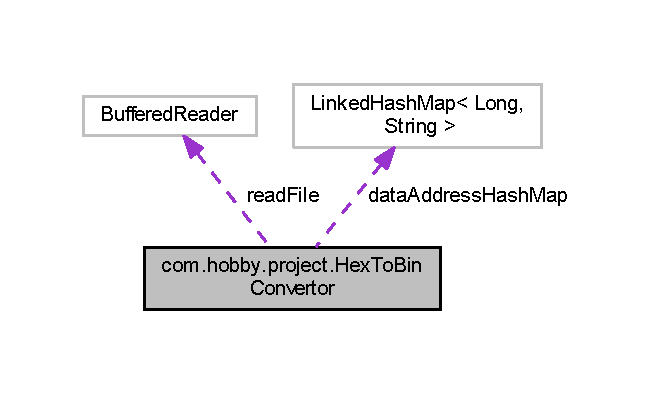
\includegraphics[width=314pt]{classcom_1_1hobby_1_1project_1_1_hex_to_bin_convertor__coll__graph}
\end{center}
\end{figure}
\subsection*{Public Member Functions}
\begin{DoxyCompactItemize}
\item 
void \hyperlink{classcom_1_1hobby_1_1project_1_1_hex_to_bin_convertor_aa8274cd08e200940cfe99c93292c5aec}{read\+Hex} (String in\+Path)  throws I\+O\+Exception 
\end{DoxyCompactItemize}
\subsection*{Static Public Member Functions}
\begin{DoxyCompactItemize}
\item 
static void \hyperlink{classcom_1_1hobby_1_1project_1_1_hex_to_bin_convertor_a5b0f6478c67aa0b3f03784f306bf30e5}{main} (String\mbox{[}$\,$\mbox{]} args)
\end{DoxyCompactItemize}


\subsection{Detailed Description}
Class reads the hex file from the given path, process the hex and writes the converted binary in to the file at a location provided by the user.

\begin{DoxyAuthor}{Author}
Mallikarjun Tirlapur 
\end{DoxyAuthor}


\subsection{Member Function Documentation}
\mbox{\Hypertarget{classcom_1_1hobby_1_1project_1_1_hex_to_bin_convertor_a5b0f6478c67aa0b3f03784f306bf30e5}\label{classcom_1_1hobby_1_1project_1_1_hex_to_bin_convertor_a5b0f6478c67aa0b3f03784f306bf30e5}} 
\index{com\+::hobby\+::project\+::\+Hex\+To\+Bin\+Convertor@{com\+::hobby\+::project\+::\+Hex\+To\+Bin\+Convertor}!main@{main}}
\index{main@{main}!com\+::hobby\+::project\+::\+Hex\+To\+Bin\+Convertor@{com\+::hobby\+::project\+::\+Hex\+To\+Bin\+Convertor}}
\subsubsection{\texorpdfstring{main()}{main()}}
{\footnotesize\ttfamily static void com.\+hobby.\+project.\+Hex\+To\+Bin\+Convertor.\+main (\begin{DoxyParamCaption}\item[{String \mbox{[}$\,$\mbox{]}}]{args }\end{DoxyParamCaption})\hspace{0.3cm}{\ttfamily [static]}}

The application starting point.


\begin{DoxyParams}{Parameters}
{\em args} & \\
\hline
\end{DoxyParams}
Here is the call graph for this function\+:
\nopagebreak
\begin{figure}[H]
\begin{center}
\leavevmode
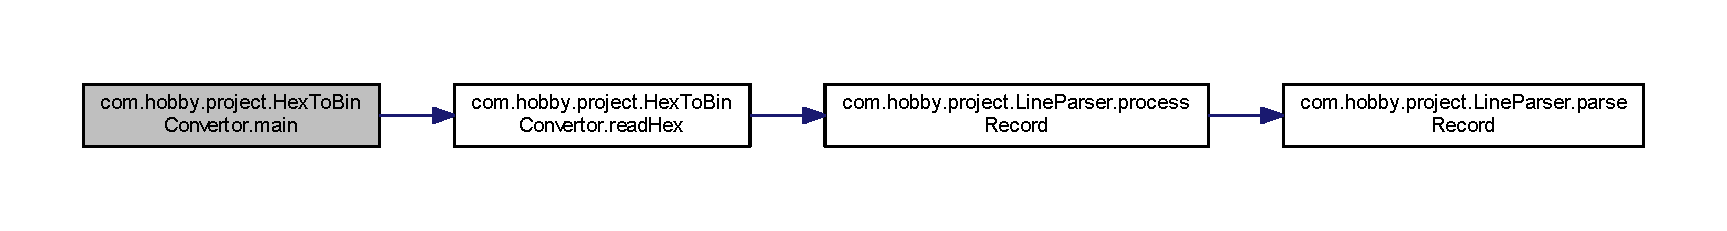
\includegraphics[width=350pt]{classcom_1_1hobby_1_1project_1_1_hex_to_bin_convertor_a5b0f6478c67aa0b3f03784f306bf30e5_cgraph}
\end{center}
\end{figure}
\mbox{\Hypertarget{classcom_1_1hobby_1_1project_1_1_hex_to_bin_convertor_aa8274cd08e200940cfe99c93292c5aec}\label{classcom_1_1hobby_1_1project_1_1_hex_to_bin_convertor_aa8274cd08e200940cfe99c93292c5aec}} 
\index{com\+::hobby\+::project\+::\+Hex\+To\+Bin\+Convertor@{com\+::hobby\+::project\+::\+Hex\+To\+Bin\+Convertor}!read\+Hex@{read\+Hex}}
\index{read\+Hex@{read\+Hex}!com\+::hobby\+::project\+::\+Hex\+To\+Bin\+Convertor@{com\+::hobby\+::project\+::\+Hex\+To\+Bin\+Convertor}}
\subsubsection{\texorpdfstring{read\+Hex()}{readHex()}}
{\footnotesize\ttfamily void com.\+hobby.\+project.\+Hex\+To\+Bin\+Convertor.\+read\+Hex (\begin{DoxyParamCaption}\item[{String}]{in\+Path }\end{DoxyParamCaption}) throws I\+O\+Exception}

Hex file is read and inserted line by line into hash table and processed.


\begin{DoxyParams}{Parameters}
{\em in\+Path} & local path to hex file \\
\hline
\end{DoxyParams}
Here is the call graph for this function\+:
\nopagebreak
\begin{figure}[H]
\begin{center}
\leavevmode
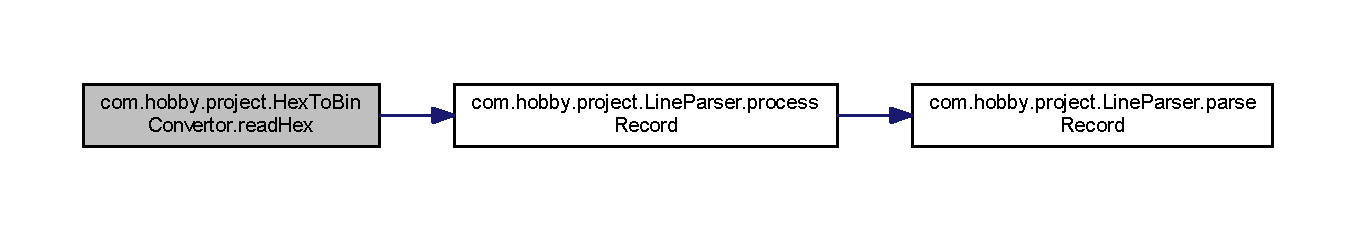
\includegraphics[width=350pt]{classcom_1_1hobby_1_1project_1_1_hex_to_bin_convertor_aa8274cd08e200940cfe99c93292c5aec_cgraph}
\end{center}
\end{figure}
Here is the caller graph for this function\+:
\nopagebreak
\begin{figure}[H]
\begin{center}
\leavevmode
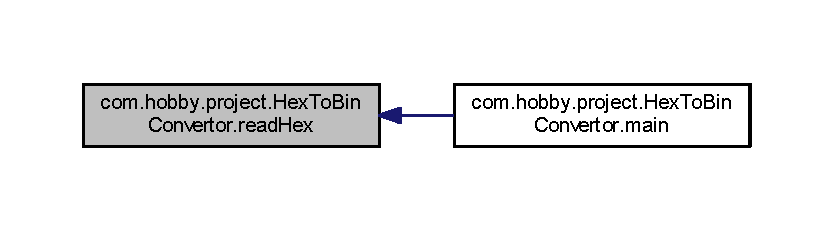
\includegraphics[width=350pt]{classcom_1_1hobby_1_1project_1_1_hex_to_bin_convertor_aa8274cd08e200940cfe99c93292c5aec_icgraph}
\end{center}
\end{figure}


The documentation for this class was generated from the following file\+:\begin{DoxyCompactItemize}
\item 
C\+:/mallik/javaproject/src/com/hobby/project/Hex\+To\+Bin\+Convertor.\+java\end{DoxyCompactItemize}

\hypertarget{classcom_1_1hobby_1_1project_1_1_line_parser}{}\section{com.\+hobby.\+project.\+Line\+Parser Class Reference}
\label{classcom_1_1hobby_1_1project_1_1_line_parser}\index{com.\+hobby.\+project.\+Line\+Parser@{com.\+hobby.\+project.\+Line\+Parser}}
\subsection*{Public Member Functions}
\begin{DoxyCompactItemize}
\item 
Linked\+Hash\+Map$<$ Long, String $>$ \hyperlink{classcom_1_1hobby_1_1project_1_1_line_parser_a6772015da2caff24e4d3c94589b1a5ff}{process\+Record} (Linked\+Hash\+Map$<$ Integer, String $>$ ln\+Tbl)
\item 
\hyperlink{classcom_1_1hobby_1_1project_1_1_record}{Record} \hyperlink{classcom_1_1hobby_1_1project_1_1_line_parser_aefe344a1777568d60dd3dc90bb5c02d2}{parse\+Record} (String record)
\end{DoxyCompactItemize}
\subsection*{Public Attributes}
\begin{DoxyCompactItemize}
\item 
\mbox{\Hypertarget{classcom_1_1hobby_1_1project_1_1_line_parser_a8082146904ae10b2d6c6abba5a351633}\label{classcom_1_1hobby_1_1project_1_1_line_parser_a8082146904ae10b2d6c6abba5a351633}} 
long {\bfseries Start\+Address}
\end{DoxyCompactItemize}


\subsection{Detailed Description}
Class parses each line from the hex file to fetch address and data which are then inserted into the hash table. Parsing is carried as per the intel hexadecimal object file format specification.

\begin{DoxyAuthor}{Author}
Mallikarjun Tirlapur 
\end{DoxyAuthor}


\subsection{Member Function Documentation}
\mbox{\Hypertarget{classcom_1_1hobby_1_1project_1_1_line_parser_aefe344a1777568d60dd3dc90bb5c02d2}\label{classcom_1_1hobby_1_1project_1_1_line_parser_aefe344a1777568d60dd3dc90bb5c02d2}} 
\index{com\+::hobby\+::project\+::\+Line\+Parser@{com\+::hobby\+::project\+::\+Line\+Parser}!parse\+Record@{parse\+Record}}
\index{parse\+Record@{parse\+Record}!com\+::hobby\+::project\+::\+Line\+Parser@{com\+::hobby\+::project\+::\+Line\+Parser}}
\subsubsection{\texorpdfstring{parse\+Record()}{parseRecord()}}
{\footnotesize\ttfamily \hyperlink{classcom_1_1hobby_1_1project_1_1_record}{Record} com.\+hobby.\+project.\+Line\+Parser.\+parse\+Record (\begin{DoxyParamCaption}\item[{String}]{record }\end{DoxyParamCaption})}

Parses each record and updates the record fields of the class \hyperlink{classcom_1_1hobby_1_1project_1_1_record}{Record}.


\begin{DoxyParams}{Parameters}
{\em record} & record is a line from the hex file which starts with \char`\"{}\+:\char`\"{}\\
\hline
\end{DoxyParams}
\begin{DoxyReturn}{Returns}
instance of \hyperlink{classcom_1_1hobby_1_1project_1_1_record}{Record}. 
\end{DoxyReturn}
Here is the caller graph for this function\+:
\nopagebreak
\begin{figure}[H]
\begin{center}
\leavevmode
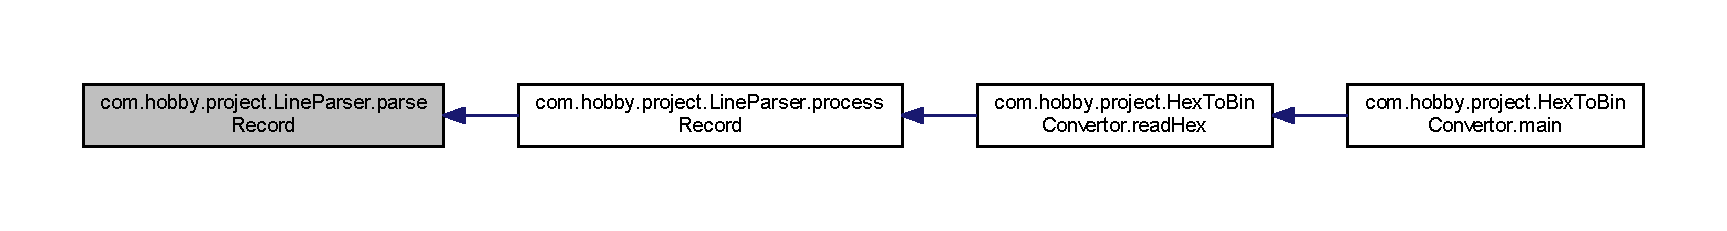
\includegraphics[width=350pt]{classcom_1_1hobby_1_1project_1_1_line_parser_aefe344a1777568d60dd3dc90bb5c02d2_icgraph}
\end{center}
\end{figure}
\mbox{\Hypertarget{classcom_1_1hobby_1_1project_1_1_line_parser_a6772015da2caff24e4d3c94589b1a5ff}\label{classcom_1_1hobby_1_1project_1_1_line_parser_a6772015da2caff24e4d3c94589b1a5ff}} 
\index{com\+::hobby\+::project\+::\+Line\+Parser@{com\+::hobby\+::project\+::\+Line\+Parser}!process\+Record@{process\+Record}}
\index{process\+Record@{process\+Record}!com\+::hobby\+::project\+::\+Line\+Parser@{com\+::hobby\+::project\+::\+Line\+Parser}}
\subsubsection{\texorpdfstring{process\+Record()}{processRecord()}}
{\footnotesize\ttfamily Linked\+Hash\+Map$<$Long, String$>$ com.\+hobby.\+project.\+Line\+Parser.\+process\+Record (\begin{DoxyParamCaption}\item[{Linked\+Hash\+Map$<$ Integer, String $>$}]{ln\+Tbl }\end{DoxyParamCaption})}

Each line is processed and based on the type of the record, memory load address is determined.


\begin{DoxyParams}{Parameters}
{\em ln\+Tbl} & hash table consisting of keys -\/ line number and values -\/ string record \\
\hline
\end{DoxyParams}
\begin{DoxyReturn}{Returns}
linked hash table containing memory load address and bin data 
\end{DoxyReturn}
Here is the call graph for this function\+:
\nopagebreak
\begin{figure}[H]
\begin{center}
\leavevmode
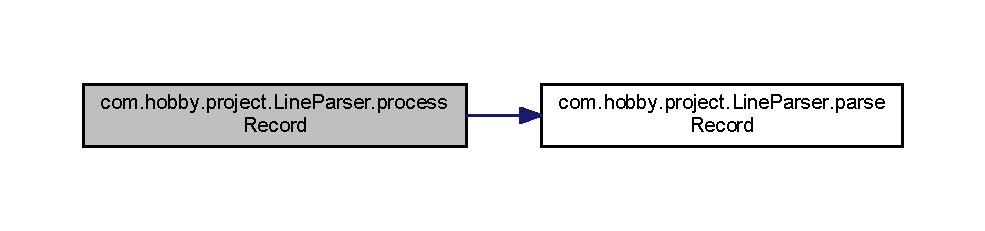
\includegraphics[width=350pt]{classcom_1_1hobby_1_1project_1_1_line_parser_a6772015da2caff24e4d3c94589b1a5ff_cgraph}
\end{center}
\end{figure}
Here is the caller graph for this function\+:
\nopagebreak
\begin{figure}[H]
\begin{center}
\leavevmode
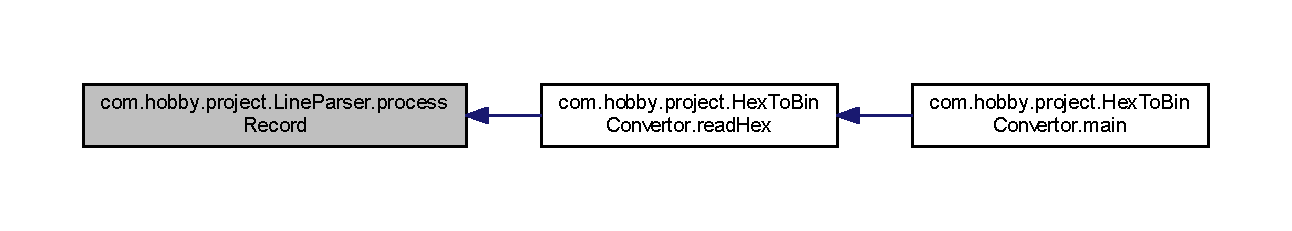
\includegraphics[width=350pt]{classcom_1_1hobby_1_1project_1_1_line_parser_a6772015da2caff24e4d3c94589b1a5ff_icgraph}
\end{center}
\end{figure}


The documentation for this class was generated from the following file\+:\begin{DoxyCompactItemize}
\item 
C\+:/mallik/javaproject/src/com/hobby/project/Line\+Parser.\+java\end{DoxyCompactItemize}

\hypertarget{classcom_1_1hobby_1_1project_1_1_record}{}\section{com.\+hobby.\+project.\+Record Class Reference}
\label{classcom_1_1hobby_1_1project_1_1_record}\index{com.\+hobby.\+project.\+Record@{com.\+hobby.\+project.\+Record}}
\subsection*{Public Attributes}
\begin{DoxyCompactItemize}
\item 
\mbox{\Hypertarget{classcom_1_1hobby_1_1project_1_1_record_addb0d0dba541731a24271f92a2d59ee4}\label{classcom_1_1hobby_1_1project_1_1_record_addb0d0dba541731a24271f92a2d59ee4}} 
int {\bfseries rec\+Len}
\item 
\mbox{\Hypertarget{classcom_1_1hobby_1_1project_1_1_record_af9dfbe833f4b9ee6864c509e985ca386}\label{classcom_1_1hobby_1_1project_1_1_record_af9dfbe833f4b9ee6864c509e985ca386}} 
String {\bfseries load\+Offset}
\item 
\mbox{\Hypertarget{classcom_1_1hobby_1_1project_1_1_record_a4a2b733db875d2106ca5bd07a6364333}\label{classcom_1_1hobby_1_1project_1_1_record_a4a2b733db875d2106ca5bd07a6364333}} 
int {\bfseries rec\+Typ}
\item 
\mbox{\Hypertarget{classcom_1_1hobby_1_1project_1_1_record_a51859e076f3924144e00a1eff523ba46}\label{classcom_1_1hobby_1_1project_1_1_record_a51859e076f3924144e00a1eff523ba46}} 
String {\bfseries data\+Bytes}
\end{DoxyCompactItemize}
\subsection*{Static Public Attributes}
\begin{DoxyCompactItemize}
\item 
\mbox{\Hypertarget{classcom_1_1hobby_1_1project_1_1_record_a0c0ea01eacfe990cae84167a2be703c1}\label{classcom_1_1hobby_1_1project_1_1_record_a0c0ea01eacfe990cae84167a2be703c1}} 
static final String {\bfseries rec\+Mark} = \char`\"{}\+:\char`\"{}
\end{DoxyCompactItemize}


\subsection{Detailed Description}
\begin{DoxyAuthor}{Author}
Mallikarjun Tirlapur 
\end{DoxyAuthor}


The documentation for this class was generated from the following file\+:\begin{DoxyCompactItemize}
\item 
C\+:/mallik/javaproject/src/com/hobby/project/Record.\+java\end{DoxyCompactItemize}

\hypertarget{classcom_1_1hobby_1_1project_1_1_records_position}{}\section{com.\+hobby.\+project.\+Records\+Position Class Reference}
\label{classcom_1_1hobby_1_1project_1_1_records_position}\index{com.\+hobby.\+project.\+Records\+Position@{com.\+hobby.\+project.\+Records\+Position}}
\subsection*{Static Public Attributes}
\begin{DoxyCompactItemize}
\item 
\mbox{\Hypertarget{classcom_1_1hobby_1_1project_1_1_records_position_ad3638141f29de29d0f8e5268c856716d}\label{classcom_1_1hobby_1_1project_1_1_records_position_ad3638141f29de29d0f8e5268c856716d}} 
static final int {\bfseries start\+Code\+Pos} = 0
\item 
\mbox{\Hypertarget{classcom_1_1hobby_1_1project_1_1_records_position_a8f3c6a7dafaf8f6ff50bc2940dccb21b}\label{classcom_1_1hobby_1_1project_1_1_records_position_a8f3c6a7dafaf8f6ff50bc2940dccb21b}} 
static final int {\bfseries byte\+Count\+Pos} = start\+Code\+Pos + 1
\item 
\mbox{\Hypertarget{classcom_1_1hobby_1_1project_1_1_records_position_a1a31c1acf28c346fda16420019e03a72}\label{classcom_1_1hobby_1_1project_1_1_records_position_a1a31c1acf28c346fda16420019e03a72}} 
static final int {\bfseries address\+Pos} = byte\+Count\+Pos + 2
\item 
\mbox{\Hypertarget{classcom_1_1hobby_1_1project_1_1_records_position_a0227745e40b81f63e27e8b6d049855ab}\label{classcom_1_1hobby_1_1project_1_1_records_position_a0227745e40b81f63e27e8b6d049855ab}} 
static final int {\bfseries record\+Type\+Pos} = address\+Pos + 4
\item 
\mbox{\Hypertarget{classcom_1_1hobby_1_1project_1_1_records_position_a2957d25cdfa4aeaf5430d30a3c69276d}\label{classcom_1_1hobby_1_1project_1_1_records_position_a2957d25cdfa4aeaf5430d30a3c69276d}} 
static final int {\bfseries data\+Pos} = record\+Type\+Pos + 2
\end{DoxyCompactItemize}


\subsection{Detailed Description}
\begin{DoxyAuthor}{Author}
Mallikarjun Tirlapur 
\end{DoxyAuthor}


The documentation for this class was generated from the following file\+:\begin{DoxyCompactItemize}
\item 
C\+:/mallik/javaproject/src/com/hobby/project/Records\+Position.\+java\end{DoxyCompactItemize}

\hypertarget{classcom_1_1hobby_1_1project_1_1_record_type}{}\section{com.\+hobby.\+project.\+Record\+Type Class Reference}
\label{classcom_1_1hobby_1_1project_1_1_record_type}\index{com.\+hobby.\+project.\+Record\+Type@{com.\+hobby.\+project.\+Record\+Type}}
\subsection*{Static Public Attributes}
\begin{DoxyCompactItemize}
\item 
\mbox{\Hypertarget{classcom_1_1hobby_1_1project_1_1_record_type_a24e6c85c86a38ba11af14789dfdfbaaf}\label{classcom_1_1hobby_1_1project_1_1_record_type_a24e6c85c86a38ba11af14789dfdfbaaf}} 
static final int {\bfseries Data\+Record} = 0x00
\item 
\mbox{\Hypertarget{classcom_1_1hobby_1_1project_1_1_record_type_af21d7c2e8f1a55998e64bb9eae25baf6}\label{classcom_1_1hobby_1_1project_1_1_record_type_af21d7c2e8f1a55998e64bb9eae25baf6}} 
static final int {\bfseries End\+Of\+File} = 0x01
\item 
\mbox{\Hypertarget{classcom_1_1hobby_1_1project_1_1_record_type_a27afe3004dcb48b4df349511a8e5efec}\label{classcom_1_1hobby_1_1project_1_1_record_type_a27afe3004dcb48b4df349511a8e5efec}} 
static final int {\bfseries Extended\+Seg\+Address} = 0x02
\item 
\mbox{\Hypertarget{classcom_1_1hobby_1_1project_1_1_record_type_a699b1fb66bd5087eaef7f90d506da972}\label{classcom_1_1hobby_1_1project_1_1_record_type_a699b1fb66bd5087eaef7f90d506da972}} 
static final int {\bfseries Start\+Seg\+Address} = 0x03
\item 
\mbox{\Hypertarget{classcom_1_1hobby_1_1project_1_1_record_type_a8e0ca2de1d6bba283ccc1834d04a9b76}\label{classcom_1_1hobby_1_1project_1_1_record_type_a8e0ca2de1d6bba283ccc1834d04a9b76}} 
static final int {\bfseries Extended\+Linear\+Address} = 0x04
\item 
\mbox{\Hypertarget{classcom_1_1hobby_1_1project_1_1_record_type_af23773aa176dc7bd292da7fa0990946d}\label{classcom_1_1hobby_1_1project_1_1_record_type_af23773aa176dc7bd292da7fa0990946d}} 
static final int {\bfseries Start\+Linear\+Address} = 0x05
\end{DoxyCompactItemize}


\subsection{Detailed Description}
\begin{DoxyAuthor}{Author}
Mallikarjun Tirlapur 
\end{DoxyAuthor}


The documentation for this class was generated from the following file\+:\begin{DoxyCompactItemize}
\item 
C\+:/mallik/javaproject/src/com/hobby/project/Record\+Type.\+java\end{DoxyCompactItemize}

%--- End generated contents ---

% Index
\backmatter
\newpage
\phantomsection
\clearemptydoublepage
\addcontentsline{toc}{chapter}{Index}
\printindex

\end{document}
